\documentclass[tikz]{standalone}
\usepackage{ctex}
\usepackage{tikz}
\usepackage{pgfplots}
\pgfplotsset{compat=1.18}   % 使用较新版本语法
\usetikzlibrary{positioning, arrows.meta, intersections, calc, fit, backgrounds}
\usepgfplotslibrary{fillbetween}  % 用于填充区域

\begin{document}
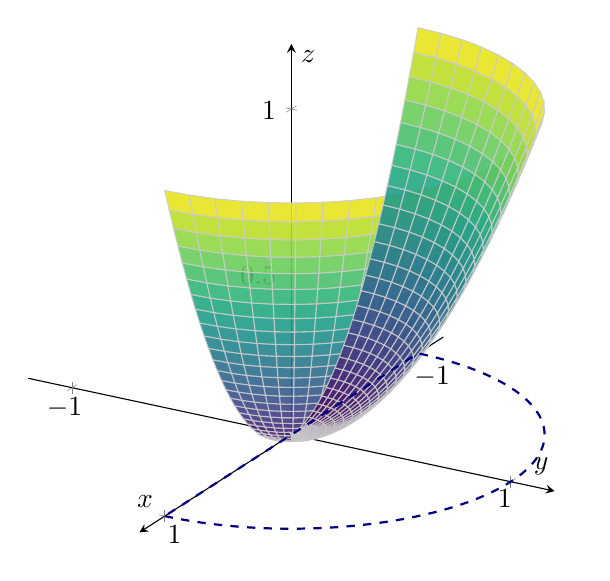
\begin{tikzpicture}
    \begin{axis}[
            view={120}{30},                     % 视角
            axis lines=center,                  % 坐标轴居中
            xlabel={$x$}, ylabel={$y$}, zlabel={$z$},
            xtick={-1,0,1}, ytick={-1,0,1}, ztick={0,0.5,1},
            width=\textwidth,   % 宽度设置为 0.8 倍版心宽
            xmin=-1.2, xmax=1.2,
            ymin=-1.2, ymax=1.2,
            zmin=0, zmax=1.2,
            colormap/viridis,
            samples=30,
            samples y=30,
            clip=false                         % 允许在区域外绘制辅助线
        ]
        % 在上半圆盘上绘制曲面 z = x^2 + y^2
        % 使用极坐标参数化：x = r*cos(theta), y = r*sin(theta), z = r^2
        % r ∈ [0,1], theta ∈ [0,180]（度）
        \addplot3[
            surf,
            domain=0:1,
            domain y=0:180,
            opacity=0.85,
            faceted color=black!20,
            fill opacity=0.9
        ] ({x*cos(y)}, {x*sin(y)}, {x^2});
        % 在 xy 平面上绘制积分区域的边界（虚线）
        \draw[thick, dashed, blue!50!black]
        (axis cs:1,0,0) arc[start angle=0, end angle=180, radius=1] -- cycle;
    \end{axis}
\end{tikzpicture}
\end{document}